\documentclass[letterpaper,11pt]{article}

% --- PAQUETES DE IDIOMA
\usepackage[spanish,mexico]{babel}
\usepackage[utf8]{inputenc}
\usepackage{csquotes}
\usepackage{iftex}

\usepackage{pdfpages}

% --- PAQUETES MATEMÁTICOS --
\usepackage{amsmath}
\usepackage{cancel}
\usepackage{mathrsfs}

% --- PAQUETES GRÁFICOS Y DE DISEÑO ---
\usepackage{graphicx}
\usepackage{float}
\usepackage{placeins}
\usepackage{subcaption}
\usepackage[table]{xcolor}
\usepackage{makecell}
\usepackage{array}
\usepackage{tikz}
\usetikzlibrary{shapes.geometric, shapes.multipart, positioning, arrows.meta, calc, shadows, decorations.pathreplacing,babel}

% --- LISTAS ---
\usepackage{enumitem}

% --- PAQUETES DE CÓDIGO ---
\usepackage{listings}
% Configuración del estilo de listings
\definecolor{codebg}{rgb}{0.95,0.95,0.95}   
\definecolor{keyword}{rgb}{0.0,0.2,0.6}     
\definecolor{comment}{rgb}{0.25,0.5,0.35}   
\definecolor{string}{rgb}{0.6,0.0,0.0}      
\definecolor{number}{rgb}{0.5,0.0,0.5}      
\definecolor{codegray}{rgb}{0.5,0.5,0.5}
\definecolor{codepurple}{rgb}{0.58,0,0.82}
\definecolor{backcolour}{rgb}{0.95,0.95,0.95}

\lstset{
  backgroundcolor=\color{backcolour},
  basicstyle=\ttfamily\small,
  keywordstyle=\color{blue}\bfseries,
  stringstyle=\color{codepurple},
  commentstyle=\color{codegray}\itshape,
  numbers=left,
  numberstyle=\tiny\color{codegray},
  frame=single,
  rulecolor=\color{black},
  breaklines=true,
  tabsize=4,
  showstringspaces=false,
  literate={á}{{\'a}}1
           {é}{{\'e}}1
           {í}{{\'i}}1
           {ó}{{\'o}}1
           {ú}{{\'u}}1
           {Á}{{\'A}}1
           {É}{{\'E}}1
           {Í}{{\'I}}1
           {Ó}{{\'O}}1
           {Ú}{{\'U}}1
           {ñ}{{\~n}}1
           {Ñ}{{\~N}}1
           {¿}{{\textquestiondown}}1
           {¡}{{\textexclamdown}}1
}

% Estilo para código en C
\lstdefinestyle{cstyle}{
  language=C,
  backgroundcolor=\color{backcolour},
  basicstyle=\ttfamily\small,
  keywordstyle=\color{blue}\bfseries,
    keywordstyle=[2]\color{yellow!70!orange}\bfseries,
    morekeywords=[2]{MPI_Init,MPI_Comm_size,MPI_Comm_rank,MPI_Send,MPI_Recv,MPI_Scatter,MPI_Gather,MPI_Bcast,MPI_Reduce,MPI_Finalize},
    emph={printf},
    emphstyle=\color{blue}\bfseries,
  stringstyle=\color{codepurple},
  commentstyle=\color{codegray}\itshape,
  numbers=left,
  numberstyle=\tiny\color{codegray},
  frame=single,
  rulecolor=\color{black},
  breaklines=true,
  tabsize=4,
  showstringspaces=false
}

% Definición del lenguaje Python para listings
\lstdefinelanguage[LAB]{Python}{
    morekeywords={False, None, True, and, as, assert, async, await, break,
                                class, continue, def, del, elif, else, except, finally,
                                for, from, global, if, import, in, is, lambda, nonlocal,
                                not, or, pass, raise, return, try, while, with, yield,
                                machine, Pin, PWM, ADC, Timer, sleep_ms, sleep_us},
    morecomment=[l]{\#},
    morestring=[b]",
    morestring=[b]',
    sensitive=true
}

% Estilo para salidas de consola/terminal
\lstdefinestyle{output}{
  backgroundcolor=\color{black!5},
  basicstyle=\ttfamily\footnotesize,
  numbers=none,
  frame=single,
  rulecolor=\color{black!30},
  breaklines=true,
  tabsize=4,
  showstringspaces=false,
  xleftmargin=0.5cm,
  xrightmargin=0.5cm
}

% --- ESTILOS PARA DIAGRAMAS DE FLUJO (TIKZ) ---
\tikzset{
  startstop/.style={rectangle, rounded corners, minimum width=3cm, minimum height=1cm,text centered, draw=black, fill=red!30},
  process/.style={rectangle, minimum width=3cm, minimum height=1cm, text centered, draw=black, fill=orange!30},
  decision/.style={diamond, aspect=2, minimum width=3cm, minimum height=1cm, text centered, draw=black, fill=green!30},
  io/.style={trapezium, trapezium left angle=70, trapezium right angle=110, minimum width=3cm, minimum height=1cm, text centered, draw=black, fill=blue!30},
  arrow/.style={thick,->,>=stealth}
}


\definecolor{azulresultado}{HTML}{0072C6}
\definecolor{rojoacarreo}{HTML}{FF0000}

% --- RUTAS DE IMÁGENES ---
\graphicspath{{img/}{portada_img/}}

\definecolor{armblue}{RGB}{0, 113, 188}

% --- ÍNDICE CON PUNTOS ---
\usepackage{tocloft}
\renewcommand{\cftsecleader}{\cftdotfill{\cftdotsep}}

% --- CONFIGURACIÓN DE PÁGINA (GEOMETRÍA) ---
\usepackage[
    left=25mm, 
    right=25mm,
    top=35mm,
    bottom=30mm,
    headheight=77pt, 
    papersize={21.59cm,27.94cm}
]{geometry}

% --- FORMATO DE TEXTO ---
\usepackage{setspace}
\onehalfspacing
\usepackage{parskip} 
\usepackage{lipsum}  

% --- VARIABLES GLOBALES ---
\newcommand{\materia}{}

% --- ENCABEZADOS Y PIES DE PÁGINA ---
\usepackage{fancyhdr}
\pagestyle{fancy}
\fancyhf{} 
\fancyhead[L]{
\includegraphics[height=1.5cm]{portada_img/der.png}}
\fancyhead[R]{
\includegraphics[height=1.5cm]{portada_img/izq.png}}
\fancyfoot[C]{\thepage} 
\renewcommand{\headrulewidth}{0.4pt} 
\renewcommand{\footrulewidth}{0pt}  

% --- BIBLIOGRAFÍA ---
\usepackage[backend=biber, style=apa, sortcites, url=true]{biblatex}
\addbibresource{referencias.bib}

% --- HIPERVÍNCULOS ---
\usepackage{hyperref}
\hypersetup{
    colorlinks=true,
    linkcolor=blue,
    citecolor=blue,
    filecolor=magenta,
    urlcolor=cyan
}

\begin{document}

\input{portada.tex}

\newpage
{\hypersetup{linkcolor=black}\tableofcontents}


\newpage

\setcounter{page}{1}
\singlespacing

\section{LLM Utilizado }

La IA utilizada para este analisis fue 
\textbf{Gemini 3.1 Pro Alto razonamiento}, esto por su capacidad de entregar
graficos y poder tener una mejor comprension de los datos, ademas de que tiene un mejor entendimiento del lenguaje natural y puede generar respuestas mas coherentes y precisas.

\section{Prompt Completo para la IA}

\begin{quote}
  Actúa como un Analista de Datos.
  Te voy a proporcionar un documento llamado titanic.tab, sobre pasajeros, delimitado por tablas, que contiene las columnas status, age, sex y survived. No obstante, algunas  filas contienen valores d y un salto con la palabra class, asi que para eso, necesito que por favor, ignora esas anomalías o tu mismo valores que hacer con ellas en caso que lo consideres importante, y procesa únicamente los registros.
  Tu meta es que realices un análisis completo y estructurado, siguiendo una estructura profesional, como la siguiente, donde primero:

  Proporciona el conteo total de registros válidos analizados.
  Calcula la tasa de supervivencia global del dataset.
  Después de eso tendrás que sacar lo siguiente:

  Calcula y compara la tasa de supervivencia agrupada por Clase/Status (First, Second, Third, Crew).
  Calcula y compara la tasa de supervivencia agrupada por Sexo (Male, Female).
  Calcula y compara la tasa de supervivencia agrupada por Edad (Adult, Child).
  Identifica el grupo con la mayor y la menor probabilidad de supervivencia cruzando al menos dos variables.
  En seguida tendrás que sacar lo siguiente:

  Enumera de 3 a 5 hallazgos críticos que revelen el comportamiento de los datos.
  Y para casi finalizar:

  Genera gráficos que tome estos datos y genere tres gráficas clave:
  Un gráfico de barras de supervivencia por Sexo.
  Un gráfico de barras apiladas o agrupadas de supervivencia por Status/Clase.
  Un heatmap o gráfico equivalente que muestre la correlación de supervivencia cruzando Status y Sexo.
  De esas graficas, tendrás que dar una interpretación correcta de cada una, con su respectivo análisis.

  Por ultimo:
  Cierra con un breve análisis cualitativo sobre lo que estos datos nos dicen sobre las prioridades de evacuación o rescate.

  En cada grafico, justo abajo tendra que ir su interpretacion, para que tenga un orden correcto cada analisis y cada estructura del analisis.
\end{quote}

\newpage
\section{Respuesta del modelo de IA (gemini)}

\begin{figure}[h!]
    \centering
    % Figura individual 1
    \begin{minipage}{0.45\textwidth}
        \centering
        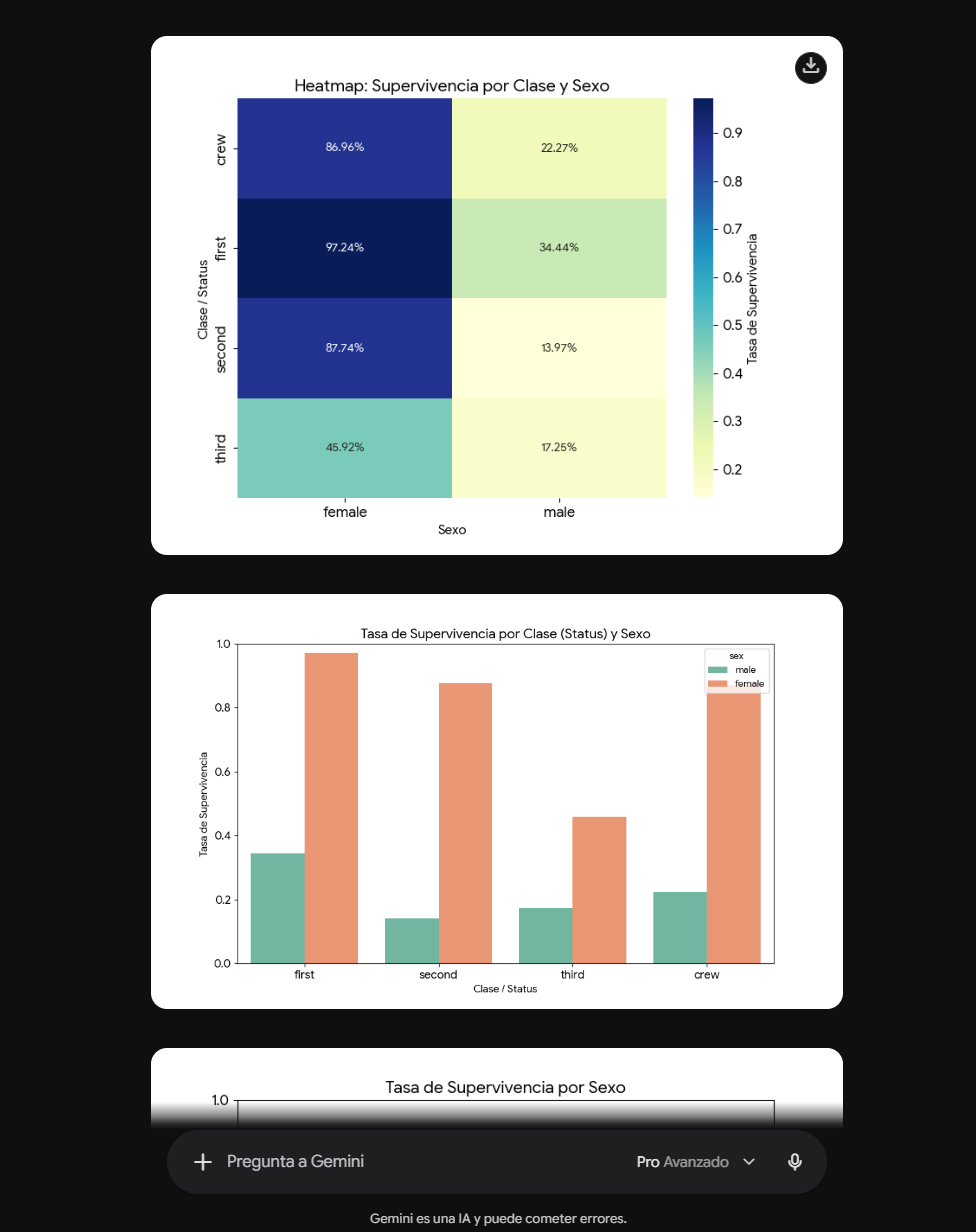
\includegraphics[width=\textwidth]{image/imagen1.png}
        \captionof{figure}{Supervivencia por clase y Sexo.}
    \end{minipage}
    \hfill
    % Figura individual 2
    \begin{minipage}{0.41\textwidth}
        \centering
        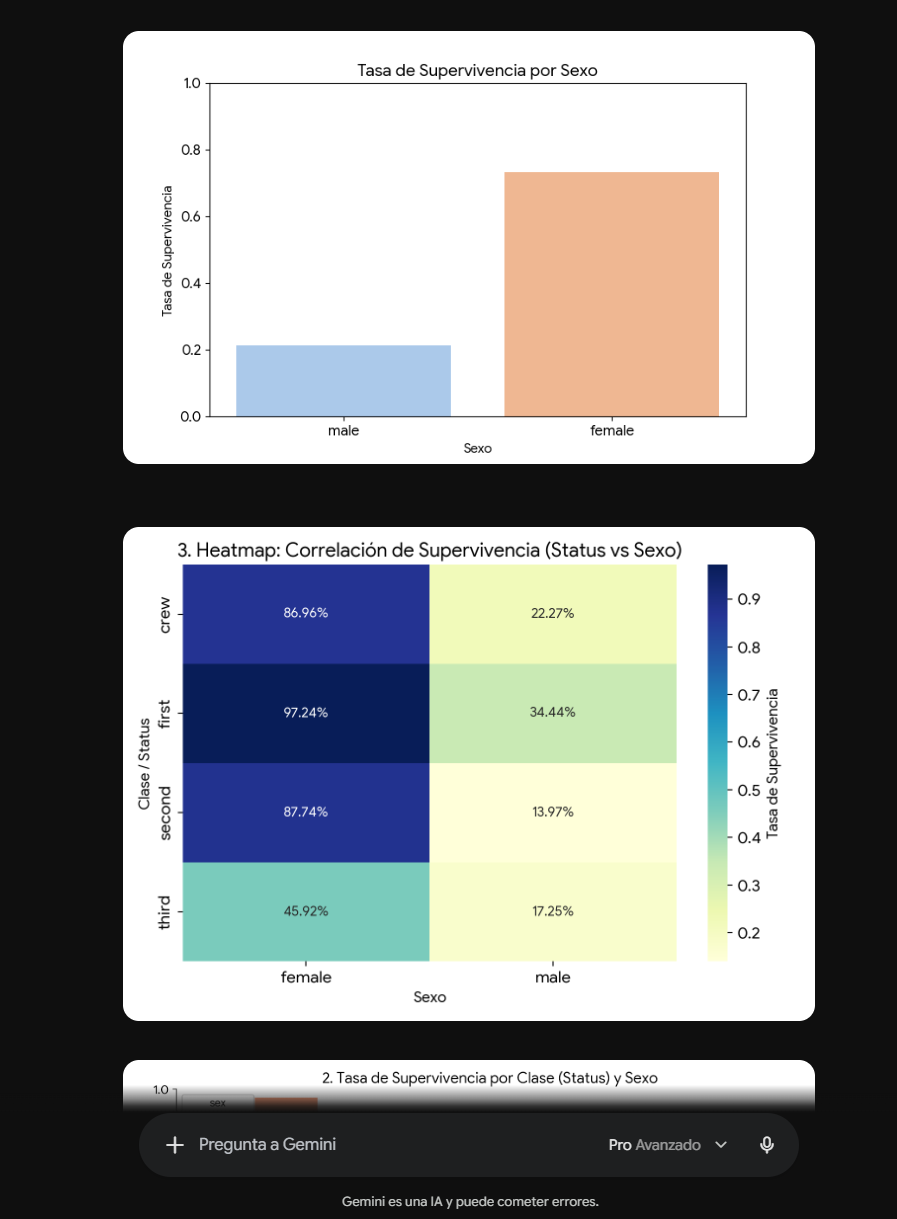
\includegraphics[width=\textwidth]{image/imagen2.png}
        \captionof{figure}{Heatmap correlacion de superviviencia}
    \end{minipage}
\end{figure}

\begin{figure}[H]
  \centering
  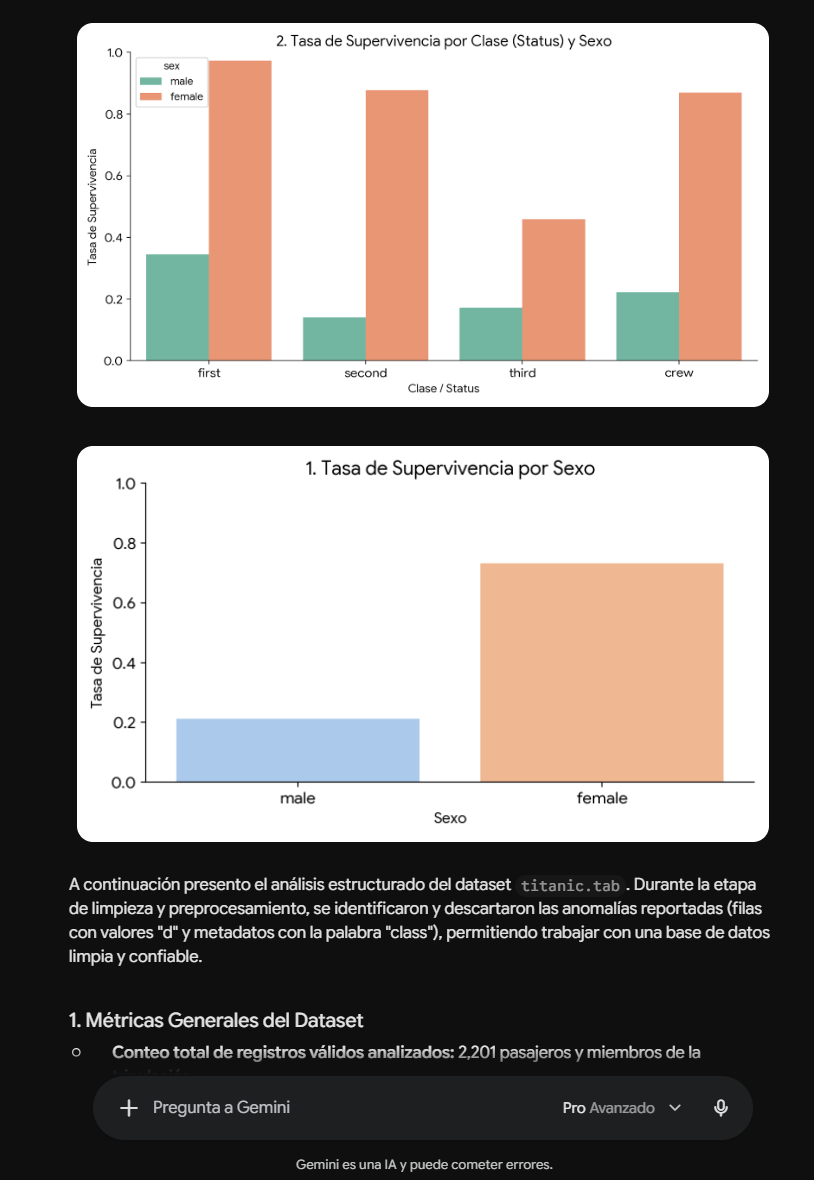
\includegraphics[width=0.35\textwidth]{image/imagen3.png}
  \caption{Supervivencia por Sexo}
\end{figure}

\newpage

A continuación presento el análisis estructurado del dataset \texttt{titanic.tab}. Durante la etapa de limpieza y preprocesamiento, se identificaron y descartaron las anomalías reportadas (filas con valores ``d'' y metadatos con la palabra ``class''), permitiendo trabajar con una base de datos limpia y confiable.

\subsection{Métricas Generales del Dataset}
\begin{itemize}
    \item \textbf{Conteo total de registros válidos analizados:} 2,201 pasajeros y miembros de la tripulación.
    \item \textbf{Tasa de supervivencia global del dataset:} 32.30\%.
\end{itemize}

\subsection{Tasa de Supervivencia Agrupada (Descriptivo)}

\subsection*{Por Clase/Status Socioeconómico:}
\begin{itemize}
    \item \textbf{First (Primera):} 62.46\%
    \item \textbf{Second (Segunda):} 41.40\%
    \item \textbf{Third (Tercera):} 25.21\%
    \item \textbf{Crew (Tripulación):} 23.95\%
\end{itemize}

\subsection*{Por Sexo:}
\begin{itemize}
    \item \textbf{Female (Mujeres):} 73.19\%
    \item \textbf{Male (Hombres):} 21.20\%
\end{itemize}

\subsection*{Por Edad:}
\begin{itemize}
    \item \textbf{Child (Niños):} 52.29\%
    \item \textbf{Adult (Adultos):} 31.26\%
\end{itemize}

\subsection{Extremos de Probabilidad (Cruce de Variables)}
Cruzando las variables de Status y Sexo, se identificaron los siguientes grupos demográficos extremos:
\begin{itemize}
    \item \textbf{Grupo con mayor probabilidad de supervivencia:} Mujeres de Primera Clase (\textit{First - Female}), con una tasa extraordinaria del 97.24\%.
    \item \textbf{Grupo con menor probabilidad de supervivencia:} Hombres de Segunda Clase (\textit{Second - Male}), con apenas un 13.97\%.
\end{itemize}

\subsection{Hallazgos Críticos del Comportamiento de los Datos}
\begin{enumerate}
    \item \textbf{El género como el predictor más fuerte:} El sexo de los pasajeros dictaminó drásticamente el destino. Las mujeres tuvieron más de tres veces la probabilidad de sobrevivir en comparación con los hombres (73.19\% frente a 21.20\%), demostrando una fuerte aplicación de políticas de prioridad de abordaje.
    \item \textbf{Correlación directa entre estatus y vida:} La supervivencia cae de manera escalonada y consistente conforme se desciende en el nivel socioeconómico de los pasajeros. Ser de primera clase otorgó casi el triple de oportunidades de sobrevivir frente a un miembro de la tripulación o un pasajero de tercera clase.
    \item \textbf{La paradoja del hombre de segunda clase:} Aunque se esperaría que la tercera clase o la tripulación tuvieran las peores métricas en todos los cruces demográficos, fueron los hombres de segunda clase quienes registraron la menor supervivencia de todo el barco (13.97\%). Esto sugiere que los hombres de esta clase acataron de forma mucho más estricta la orden de ``mujeres y niños primero'' y se quedaron atrás, mientras que un porcentaje mayor de tripulantes y pasajeros de tercera clase lograron encontrar rutas alternativas hacia los botes.
    \item \textbf{Prioridad generacional moderada por la clase:} Aunque los niños (52.29\%) sobrevivieron en mayor medida que los adultos (31.26\%), su tasa global es significativamente menor que la de las mujeres. Esto revela que el estatus socioeconómico de las familias de tercera clase afectó negativamente y limitó el rescate de los niños que pertenecían a ese estrato.
\end{enumerate}

\subsection{Análisis Gráfico e Interpretaciones}
(\textit{Las gráficas generadas a partir del procesamiento de los datos se visualizan en los bloques de resultados del código original}).

\subsection*{Interpretación del Gráfico 1: Tasa de Supervivencia por Sexo}
Este gráfico de barras simple expone visualmente el abismo existente en la política de rescate. La barra correspondiente a las mujeres supera el 70\%, mientras que la de los hombres apenas rebasa la línea del 20\%. Esto confirma matemáticamente que el principal criterio de selección en las primeras fases del desastre estuvo estrictamente dictado por el género.

\subsection*{Interpretación del Gráfico 2: Tasa de Supervivencia por Clase (Status) y Sexo}
El gráfico de barras agrupadas demuestra cómo interactuaron la jerarquía social y el género. Se observa que la ventaja de ser mujer se mantiene en todas las clases, pero sufre una caída drástica en la tercera clase (apenas por debajo del 50\%). Así mismo, muestra visualmente la anomalía mencionada en los hallazgos: la barra de supervivencia de los hombres de segunda clase (la más baja de todo el gráfico) se encuentra visiblemente por debajo de los hombres de tercera clase y de la tripulación, rompiendo la tendencia descendente que sí siguen las mujeres.

\subsection*{Interpretación del Gráfico 3: Heatmap (Correlación de Supervivencia cruzando Status y Sexo)}
El mapa de calor sintetiza la gravedad de la distribución demográfica. Las celdas más oscuras (mayor supervivencia) se concentran exclusivamente en el cuadrante superior izquierdo (Mujeres de Primera y Segunda clase, con 97.24\% y 87.74\%). A medida que la mirada se desplaza hacia la derecha (Hombres) y hacia abajo (Tercera Clase y Tripulación), los tonos se vuelven mucho más claros, culminando en la tasa letal del 13.97\% para los hombres de segunda clase. Este gráfico ilustra perfectamente que para tener garantías de vida en este evento, no bastaba con cumplir un solo criterio (ser mujer o tener dinero), sino la intersección de ambos.

\subsection{Conclusión Cualitativa: Prioridades de Evacuación y Rescate}
Los datos documentan una logística de evacuación gobernada por un cruce fatal entre el protocolo marítimo idealista (``Mujeres y niños primero'') y una rígida segregación arquitectónica y socioeconómica.

Las métricas sugieren fuertemente que la evacuación no fue un proceso de rescate universal y caótico, sino uno altamente estructurado donde las prioridades estuvieron dictadas por la ubicación de los camarotes y el estatus social. La primera clase, con mejor acceso a las cubiertas superiores y asistencia temprana, pudo asegurar a sus mujeres e incluso a una porción moderada de sus hombres. Por otro lado, la altísima mortalidad en la tercera clase y en la tripulación habla de fallas sistémicas, barreras físicas y una alarmante falta de priorización para advertir y movilizar a la base de la pirámide social del barco, condenando a la gran mayoría por su incapacidad material para alcanzar un bote salvavidas a tiempo.

\section{Conversacion con la IA}
\url{https://share.gemini.google/aNWxzv42x0dj}



% Impresión Referencias
\nocite{*}
\printbibliography[heading=bibintoc, title={Referencias}]

\end{document}